\aberturaModulo{UNIDADE I}{TERRITÓRIO E ECOSSISTEMAS}{Encontros 1 a 6 $\bullet$ Base da AV1 (30\%) e Leitura Territorial da AV3}{%
Esta unidade estabelece os fundamentos teóricos, econômicos e territoriais do empreendedorismo tecnológico. Ao longo de seis encontros, o estudante transita da firma inovadora individual para a compreensão sistêmica do território como construção social e institucional capaz de gerar, reter ou drenar valor tecnológico.
\begin{itemize}[leftmargin=1.4em, itemsep=2pt, topsep=4pt]
  \item \textbf{Capítulo 1:} Empreendedorismo de Base Tecnológica e Desenvolvimento Territorial (Schumpeter, Kuhn, Dosi, Mazzucato e Milton Santos).
  \item \textbf{Capítulo 2:} Estruturas de Mercado, Barreiras de Entrada e Aglomerações Produtivas (Porter, Índice HHI e Eficiência Coletiva em APLs).
  \item \textbf{Capítulo 3:} Ecossistemas Empreendedores e Sistemas Regionais de Inovação (Isenberg, Stam \& van de Ven e Proximidades de Boschma).
  \item \textbf{Capítulo 4:} Governança Territorial da Inovação e Políticas Públicas de CT\&I (Hélice Tríplice à Quíntupla e Estado Empreendedor).
  \item \textbf{Capítulo 5:} Empreendedorismo Social e Negócios de Impacto Territorial (Espectro de Impacto, Matriz PCDO e Teoria da Mudança).
  \item \textbf{Capítulo 6:} Inovação Social, Economia Solidária, Bioeconomia e Indicações Geográficas (Dagnino, Tecnologia Social e INPI).
\end{itemize}
}

\chapter{Empreendedorismo de Base Tecnológica e Desenvolvimento Territorial}
\tagAV{AV1 (30\%)}\ \tagTerritorio

\begin{capObjetivos}
Ao concluir este capítulo, você será capaz de:
\begin{itemize}[leftmargin=1.4em, itemsep=2pt]
  \item Distinguir Empresas de Base Tecnológica (EBTs) de negócios convencionais a partir de intensidade de P\&D, ativos intangíveis, propriedade intelectual (PI) e ciclo de maturação.
  \item Classificar empreendimentos tecnológicos segundo sua matriz produtiva e institucional (\textit{Deep Tech}, Base Digital, \textit{Spin-off} Acadêmica e Tecnologia Social/Agro).
  \item Aplicar os conceitos schumpeterianos de inovação, destruição criadora e transição entre os modelos \textit{Mark I} e \textit{Mark II} à dinâmica competitiva.
  \item Analisar paradigmas e trajetórias tecnológicas (Kuhn e Dosi), identificando mecanismos de \textit{path dependence} e aprisionamento (\textit{lock-in}).
  \item Avaliar criticamente o papel do Estado e as assimetrias do meio técnico-científico-informacional (Milton Santos) na emergência de EBTs em regiões periféricas e no Nordeste brasileiro.
\end{itemize}
\end{capObjetivos}

\begin{capRevisao}
Para acompanhar a modelagem deste capítulo, relembre três noções básicas:
\begin{enumerate}[leftmargin=1.4em, itemsep=2pt]
  \item \textbf{Razões financeiras elementares:} participação percentual de um gasto sobre a receita operacional ($x / R_{\text{op}}$) e proporção de ativos intangíveis no ativo total ($A_{\text{int}} / A_{\text{tot}}$).
  \item \textbf{Juros compostos e desconto intertemporal:} projetos com retorno concentrado no longo prazo sofrem maior penalização quando a taxa de desconto ($r$) é elevada, pois o fator $(1+r)^{-t}$ reduz o valor presente de fluxos distantes.
  \item \textbf{Diferença entre invenção e inovação:} a invenção corresponde à criação técnica ou científica inédita; a inovação ocorre apenas quando essa solução é introduzida com sucesso econômico ou social no mercado ou no território.
\end{enumerate}
\end{capRevisao}

\etapa{3}{Fundamentação Teórica, Tipologia e Modelagem da Firma Tecnológica}

\begin{boxSimbolo}[Vocabulário Conceitual e Notação do Capítulo]
\begin{tabularx}{\linewidth}{@{}l X@{}}
  \toprule
  \textbf{Símbolo / Termo} & \textbf{Significado Analítico e Unidade} \\
  \midrule
  EBT & Empresa de Base Tecnológica (firma apoiada em conhecimento científico-tecnológico proprietário ou complexo). \\
  $I_{\text{P\&D}}$ & Intensidade de Pesquisa e Desenvolvimento: razão entre dispêndio em P\&D e receita operacional líquida (\%). \\
  $\rho_{\text{int}}$ & Razão de intangibilidade: proporção de ativos intangíveis (patentes, software, \textit{know-how}) no ativo total (adimensional ou \%). \\
  $T_{\text{mat}}$ & Ciclo de maturação tecnológica: tempo decorrido entre a prova de conceito e o ponto de equilíbrio operacional (anos). \\
  $\mu_{\text{loc}}$ & Multiplicador territorial de retenção: razão entre o valor adicionado retido no território e o aporte inicial em P\&D (adimensional). \\
  \textit{Path dependence} & Dependência de trajetória: condicionamento das escolhas tecnológicas presentes por decisões e investimentos acumulados no passado. \\
  \textit{Lock-in} & Aprisionamento tecnológico, institucional ou cognitivo em uma trajetória subótima devido a altos custos de transição. \\
  \bottomrule
\end{tabularx}
\end{boxSimbolo}

\section{O que define uma Empresa de Base Tecnológica (EBT)}

Na literatura internacional, Storey e Tether (1998) caracterizam as novas firmas de base tecnológica como empreendimentos independentes cuja vantagem competitiva deriva da exploração de conhecimento científico ou de engenharia avançada, operando geralmente em setores de alta intensidade em Pesquisa e Desenvolvimento (P\&D). Ampliando essa definição, Bailetti (2012) conceitua o empreendedorismo tecnológico como o investimento em projetos que reúnem e implantam ativos especializados e indivíduos heterogêneos, intimamente ligados a avanços no conhecimento científico e tecnológico, com o propósito de criar e capturar valor para a firma.

Diferentemente de empresas comerciais ou de serviços tradicionais, em que a barreira de entrada reside na localização comercial ou no capital de giro imediato, a EBT estrutura-se sobre quatro pilares interdependentes:

\begin{enumerate}[leftmargin=1.4em, itemsep=3pt]
  \item \textbf{Intensidade de P\&D:} alocação sistemática de recursos financeiros e horas de pessoal qualificado para resolver incertezas técnicas não triviais, frequentemente acima de $5\%$ da receita operacional líquida na fase madura e superior a $30\%$ na fase pré-operacional.
  \item \textbf{Predomínio de ativos intangíveis:} o valor econômico da organização concentra-se em algoritmos, formulações químicas, linhagens biológicas, desenhos industriais, segredos de negócio e capital humano especializado, e não em estoques físicos ou imóveis.
  \item \textbf{Proteção por Propriedade Intelectual (PI):} uso estratégico de patentes de invenção, modelos de utilidade, registros de software, cultivares ou indicações geográficas para assegurar exclusividade temporária e viabilizar o retorno sobre o risco técnico.
  \item \textbf{Ciclo longo de maturação:} intervalo prolongado entre a bancada laboratorial e a validação comercial (frequentemente de $3$ a $10$ anos em biotecnologia, novos materiais ou energia), exigindo capital paciente e governança tolerante à falha técnica.
\end{enumerate}

\begin{boxConceito}[Tipologia Operacional das EBTs no Território]
Para fins de análise estratégica e formulação de políticas públicas, as EBTs dividem-se em quatro arquétipos principais, que variam em risco técnico, velocidade de escalonamento e enraizamento territorial:
\begin{itemize}[leftmargin=1.4em, itemsep=2pt]
  \item \textbf{\textit{Deep Tech}:} empreendimentos baseados em descobertas científicas ou avanços disruptivos de engenharia (biotecnologia, fotônica, novos materiais, inteligência artificial fundamental). Apresentam alto risco tecnológico, forte proteção por patentes e ciclo longo de maturação.
  \item \textbf{Base Digital (\textit{Software-driven}):} negócios estruturados em plataformas digitais, SaaS (\textit{Software as a Service}), análise de dados e automação de processos. Exibem menor custo fixo inicial, ciclo de validação mais curto e risco predominantemente de mercado e adoção.
  \item \textbf{\textit{Spin-off} Acadêmica:} empresa originada no interior de universidades ou institutos de pesquisa para transferir comercialmente uma tecnologia desenvolvida em laboratório público ou grupo de pesquisa, mantendo vínculos formais de licenciamento de PI ou uso compartilhado de infraestrutura.
  \item \textbf{Tecnologia Social e Agroecológica/Agroindustrial:} soluções tecnológicas orientadas à resolução de gargalos produtivos, hídricos, sanitários ou ambientais em territórios específicos (como bioinsumos adaptados ao Semiárido, dessalinização solar ou processamento de cadeias da sociobiodiversidade), combinando conhecimento científico formal e saberes locais.
\end{itemize}
\end{boxConceito}

\section{Dinâmica Schumpeteriana, Paradigmas e Dependência de Trajetória}

Joseph Schumpeter rompeu com a visão estática do equilíbrio walrasiano ao posicionar a inovação como o motor endógeno do desenvolvimento econômico. Em \textit{Teoria do Desenvolvimento Econômico} (1911), Schumpeter identifica cinco formas de novas combinações produtivas: (i) introdução de um novo bem ou de uma nova qualidade de bem; (ii) introdução de um novo método de produção; (iii) abertura de um novo mercado; (iv) conquista de uma nova fonte de oferta de matérias-primas ou bens semimanufaturados; e (v) estabelecimento de uma nova organização de qualquer indústria, como a criação ou ruptura de um monopólio.

Ao longo de sua obra, o autor descreveu dois regimes distintos de inovação, posteriormente sistematizados pela literatura neo-schumpeteriana como \textbf{Mark I} e \textbf{Mark II}:

\begin{itemize}[leftmargin=1.4em, itemsep=3pt]
  \item \textbf{Schumpeter Mark I (1911):} regime marcado pelo \textit{alargamento tecnológico} (\textit{widening}). Novos entrantes liderados pelo empresário-inovador rompem estruturas estabelecidas por meio de inovações radicais, reduzindo a concentração de mercado e operando com baixa cumulatividade inicial.
  \item \textbf{Schumpeter Mark II (1942):} em \textit{Capitalismo, Socialismo e Democracia}, Schumpeter observa o \textit{aprofundamento tecnológico} (\textit{deepening}). A inovação torna-se rotinizada em departamentos internos de P\&D de grandes corporações, que acumulam vantagens de escala, financiamento e conhecimento tácito, elevando barreiras à entrada. Nesse contexto opera a \textbf{Destruição Criadora}: o processo incessante pelo qual novas tecnologias e modelos organizacionais tornam obsoletos os parques produtivos, competências e rendas monopolistas anteriores.
\end{itemize}

Para explicar por que a inovação não ocorre de forma aleatória em todas as direções, Giovanni Dosi (1982) adaptou a noção de paradigma científico de Thomas Kuhn (1962). Assim como Kuhn definiu o paradigma científico como um conjunto de problemas e métodos legitimados por uma comunidade científica durante períodos de ``ciência normal'', Dosi definiu o \textbf{paradigma tecnológico} como um modelo de solução de problemas técnicos selecionados com base em princípios das ciências naturais e em tecnologias materiais específicas (por exemplo, o paradigma do motor a combustão interna ou o paradigma do silício na microeletrônica).

Dentro de um paradigma, o progresso técnico segue uma \textbf{trajetória tecnológica} definida pelo conjunto de avanços incrementais e cumulativos ao longo de \textit{trade-offs} econômicos e técnicos relevantes. Como os retornos são crescentes com a adoção (economias de escala, efeitos de rede e aprendizado pelo uso), o sistema desenvolve \textbf{\textit{path dependence}} (dependência de trajetória): escolhas históricas contingentes passam a condicionar as opções futuras. Quando os custos de mudança tornam-se proibitivos frente a alternativas tecnicamente superiores, instala-se o \textbf{\textit{lock-in}} (aprisionamento tecnológico ou institucional).

\begin{boxFormula}[Indicadores de Intensidade Tecnológica e Retenção Territorial]
\textbf{Origem:} Indicadores derivados do Manual de Frascati (OCDE) para mensuração de P\&D, da contabilidade de intangíveis e da análise de multiplicadores regionais de inovação.

\textbf{Variáveis:}
\begin{itemize}[leftmargin=1.4em, itemsep=1pt]
  \item $G_{\text{P\&D}}$: gasto anual em pesquisa e desenvolvimento (R\$).
  \item $R_{\text{op}}$: receita operacional líquida anual (R\$).
  \item $A_{\text{int}}$: valor dos ativos intangíveis (patentes, software, P\&D ativada) (R\$).
  \item $A_{\text{tot}}$: ativo total da empresa (R\$).
  \item $\Delta Y_{\text{loc}}$: valor adicionado retido no território (salários qualificados locais, compras de fornecedores locais e impostos locais) (R\$).
\end{itemize}

\textbf{Equações operacionais:}
\[
I_{\text{P\&D}} = \frac{G_{\text{P\&D}}}{R_{\text{op}}} \times 100\%
\qquad
\rho_{\text{int}} = \frac{A_{\text{int}}}{A_{\text{tot}}} \times 100\%
\qquad
\mu_{\text{loc}} = \frac{\Delta Y_{\text{loc}}}{G_{\text{P\&D}}}
\]

\textbf{Interpretação e exemplo rápido:} Uma \textit{spin-off} de sensores agrícolas fatura $R_{\text{op}} = \reais{800.000}$, investe $G_{\text{P\&D}} = \reais{200.000}$ no ano e possui $\reais{450.000}$ em intangíveis dentro de um ativo total de $\reais{600.000}$. Sua intensidade de P\&D é $I_{\text{P\&D}} = (200.000 / 800.000) \times 100\% = 25\%$ e sua razão de intangibilidade é $\rho_{\text{int}} = (450.000 / 600.000) \times 100\% = 75\%$, valores típicos de EBT em fase de consolidação.
\end{boxFormula}

\section{Contraponto Crítico: O Estado Empreendedor e o Meio Técnico-Científico-Informacional}

A narrativa schumpeteriana clássica frequentemente mitifica o empreendedor heroico ou a grande corporação autossuficiente como fontes primárias da inovação radical. Mariana Mazzucato (2014) desmonta essa premissa ao demonstrar empiricamente que tecnologias fundacionais da economia contemporânea (internet, GPS, telas sensíveis ao toque, biotecnologia de ponta e energias renováveis) dependeram de investimentos públicos pacientes e de alto risco financiados por agências estatais antes de serem apropriadas pelo capital privado. A crítica central de Mazzucato aponta uma assimetria estrutural: enquanto os riscos das fases iniciais são socializados pelo orçamento público, os retornos financeiros da comercialização tendem a ser privatizados sem mecanismos proporcionais de retorno ao erário.

No plano geográfico, a inovação não flutua em um espaço isotrópico. Milton Santos (1996) formula o conceito de \textbf{meio técnico-científico-informacional} para descrever a fase atual de organização do espaço geográfico, na qual ciência, tecnologia e informação integram-se diretamente à materialidade do território. Contudo, a distribuição dessa infraestrutura informacional é profundamente desigual, criando \textit{luminosidades} (nós altamente conectados, dotados de universidades, banda larga de alta capacidade, capital de risco e serviços jurídicos especializados) e \textit{opacidades} (regiões periféricas com baixa densidade institucional e dependência de cadeias primárias).

Em regiões periféricas e no Nordeste brasileiro, o desafio das EBTs não se resume a gerar ideias inovadoras. O gargalo reside em superar a drenagem de talentos e patentes para centros hegemônicos, articulando pesquisa acadêmica regional (universidades estaduais e federais, institutos tecnológicos) com demandas produtivas concretas do território, como bioeconomia do Semiárido, energias renováveis, tecnologia social hídrica e cadeias agroindustriais locais.

\begin{figure}[H]
  \centering
  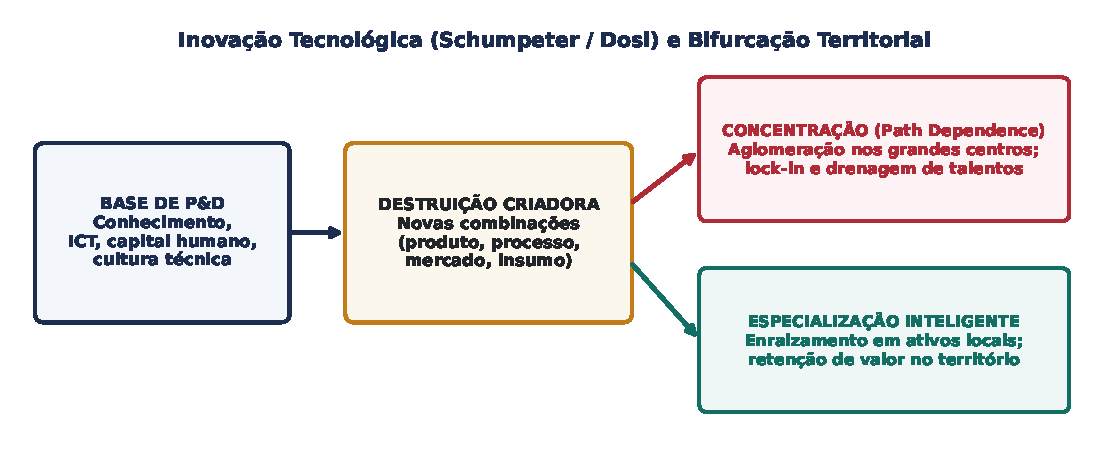
\includegraphics[width=0.94\textwidth]{figures/fig01_schumpeter_territorio.pdf}
  \caption{Integração entre dinâmica schumpeteriana (Mark I e Mark II), paradigmas e trajetórias tecnológicas (Kuhn e Dosi), intervenção pública (Mazzucato) e assimetrias do meio técnico-científico-informacional (Milton Santos).}
  \label{fig:schumpeter_territorio}
\end{figure}

\etapa{4}{Estudos de Caso e Aplicações Passo a Passo}

\begin{boxExemplo}{1}{Diagnóstico de EBT em Bioeconomia no Semiárido Baiano}
\passoEnunciado{Uma \textit{spin-off} acadêmica sediada em Feira de Santana (BA) desenvolve biofertilizantes encapsulados a partir de resíduos da mandiocultura. No último exercício fiscal, a empresa registrou receita operacional líquida de $\reais{1.200.000}$, despesas com P\&D de $\reais{270.000}$, ativos intangíveis avaliados em $\reais{960.000}$ (patente depositada no INPI e banco de cepas microbianas) e ativo imobilizado físico de $\reais{240.000}$.}
\passoDados{$R_{\text{op}} = \reais{1.200.000}$; $G_{\text{P\&D}} = \reais{270.000}$; $A_{\text{int}} = \reais{960.000}$; $A_{\text{imob}} = \reais{240.000}$.}
\passoPedido{Calcular a intensidade de P\&D ($I_{\text{P\&D}}$), a razão de intangibilidade ($\rho_{\text{int}}$) e classificar o empreendimento segundo a tipologia de EBTs.}
\passoMetodo{Aplicação das razões de intensidade tecnológica ($I_{\text{P\&D}} = G_{\text{P\&D}} / R_{\text{op}}$) e de estrutura patrimonial ($A_{\text{tot}} = A_{\text{int}} + A_{\text{imob}}$ e $\rho_{\text{int}} = A_{\text{int}} / A_{\text{tot}}$), seguida de enquadramento tipológico segundo Storey e Tether (1998) e Bailetti (2012).}
\passoContas{
  \begin{enumerate}[leftmargin=1.4em, itemsep=2pt]
    \item Cálculo do ativo total:
    \[
    A_{\text{tot}} = A_{\text{int}} + A_{\text{imob}} = 960.000 + 240.000 = \reais{1.200.000}
    \]
    \item Cálculo da intensidade de P\&D:
    \[
    I_{\text{P\&D}} = \frac{270.000}{1.200.000} \times 100\% = 0{,}225 \times 100\% = 22{,}5\%
    \]
    \item Cálculo da razão de intangibilidade:
    \[
    \rho_{\text{int}} = \frac{960.000}{1.200.000} \times 100\% = 0{,}80 \times 100\% = 80{,}0\%
    \]
  \end{enumerate}
}
\passoResposta{$I_{\text{P\&D}} = 22{,}5\%$ e $\rho_{\text{int}} = 80{,}0\%$. Trata-se de uma \textit{Spin-off} Acadêmica com perfil híbrido de \textit{Deep Tech} biotecnológica e Tecnologia Agroindustrial territorialmente enraizada.}
\passoVerificacao{Uma intensidade de P\&D de $22{,}5\%$ supera em mais de quatro vezes o limiar clássico de $5\%$ para setores de alta tecnologia, e $80\%$ do patrimônio está ancorado em conhecimento protegido. O resultado é consistente com uma EBT em estágio de validação de mercado e exige garantias financeiras baseadas em recebíveis ou subvenção, pois o baixo imobilizado limita o acesso a crédito bancário convencional.}
\end{boxExemplo}

\begin{boxExemplo}{2}{Transição Mark I para Mark II e Valor Presente do Ciclo de Maturação}
\passoEnunciado{Considere dois projetos de inovação em sensores ambientais: o Projeto A (regime \textit{Mark I}, startup independente) exige aporte único inicial de $\reais{300.000}$ em $t=0$ e gera um fluxo líquido único de $\reais{520.000}$ em $t=4$ anos após a certificação; o Projeto B (regime \textit{Mark II}, divisão de P\&D de empresa consolidada com rede comercial pronta) exige $\reais{300.000}$ em $t=0$ e gera fluxo líquido único de $\reais{460.000}$ em $t=2$ anos. A taxa mínima de atratividade (custo de oportunidade do capital) é de $12\%$ ao ano.}
\passoDados{$I_0 = \reais{300.000}$; $F_A = \reais{520.000}$ em $t_A = 4$; $F_B = \reais{460.000}$ em $t_B = 2$; $r = 0{,}12$ a.a.}
\passoPedido{Calcular o Valor Presente Líquido (VPL) de cada regime e analisar por que o ciclo longo penaliza o entrante \textit{Mark I}.}
\passoMetodo{Desconto intertemporal simples em período único: $\text{VPL} = \frac{F_t}{(1+r)^t} - I_0$.}
\passoContas{
  \begin{enumerate}[leftmargin=1.4em, itemsep=2pt]
    \item Fator de desconto para $t=4$ a $12\%$ a.a.:
    \[
    (1 + 0{,}12)^4 = 1{,}12^2 \times 1{,}12^2 = 1{,}2544 \times 1{,}2544 = 1{,}57351936
    \]
    \item VPL do Projeto A (\textit{Mark I}):
    \[
    \text{VPL}_A = \frac{520.000}{1{,}57351936} - 300.000 = 330.469{,}40 - 300.000 = \reais{30.469{,}40}
    \]
    \item Fator de desconto para $t=2$ a $12\%$ a.a.:
    \[
    (1 + 0{,}12)^2 = 1{,}2544
    \]
    \item VPL do Projeto B (\textit{Mark II}):
    \[
    \text{VPL}_B = \frac{460.000}{1{,}2544} - 300.000 = 366.709{,}18 - 300.000 = \reais{66.709{,}18}
    \]
  \end{enumerate}
}
\passoResposta{$\text{VPL}_A = \reais{30.469{,}40}$ e $\text{VPL}_B = \reais{66.709{,}18}$. Embora o retorno nominal de A seja maior ($\reais{520.000}$ contra $\reais{460.000}$), o projeto \textit{Mark II} apresenta VPL mais que dobrado devido à redução do ciclo de maturação pela metade.}
\passoVerificacao{O cálculo evidencia a vantagem estrutural das grandes empresas no regime \textit{Mark II}: ao disporem de canais de distribuição e escala prévia, encurtam o tempo até o mercado. Para que startups \textit{Mark I} sobrevivam com ciclos de $4$ a $8$ anos, tornam-se indispensáveis mecanismos de capital paciente, incubação e subvenção pública.}
\end{boxExemplo}

\begin{boxExemplo}{3}{Modelagem de \textit{Path Dependence} e Custo de Superação de \textit{Lock-in}}
\passoEnunciado{Uma cooperativa regional de beneficiamento de fibras naturais opera sob uma trajetória tecnológica antiga baseada em motores a diesel (Paradigma A), com custo operacional anual de $\reais{180.000}$/ano. Uma EBT local propõe um sistema híbrido solar-biomassa (Paradigma B) com custo operacional de $\reais{95.000}$/ano. Entretanto, a substituição exige investimento em novos equipamentos de $\reais{260.000}$ e retreinamento de operadores de $\reais{40.000}$ (custo total de transição $C_{\text{trans}} = \reais{300.000}$). O horizonte de planejamento da cooperativa é de apenas $3$ anos, sem financiamento subsidiado.}
\passoDados{$C_{\text{op},A} = \reais{180.000}$/ano; $C_{\text{op},B} = \reais{95.000}$/ano; $C_{\text{trans}} = \reais{300.000}$; horizonte $H = 3$ anos (sem desconto para análise de \textit{payback} simples).}
\passoPedido{Calcular a economia operacional anual, o tempo de retorno simples ($T_{\text{payback}}$) e verificar se há \textit{lock-in} no horizonte de decisão da cooperativa.}
\passoMetodo{Cálculo da economia anual $\Delta C_{\text{op}} = C_{\text{op},A} - C_{\text{op},B}$ e do tempo de retorno simples $T_{\text{payback}} = C_{\text{trans}} / \Delta C_{\text{op}}$, comparando com $H$.}
\passoContas{
  \begin{enumerate}[leftmargin=1.4em, itemsep=2pt]
    \item Economia operacional anual:
    \[
    \Delta C_{\text{op}} = 180.000 - 95.000 = \reais{85.000}\text{/ano}
    \]
    \item Economia acumulada no horizonte de $3$ anos:
    \[
    E_{3\text{ anos}} = 3 \times 85.000 = \reais{255.000}
    \]
    \item Saldo líquido em $3$ anos:
    \[
    S_3 = E_{3\text{ anos}} - C_{\text{trans}} = 255.000 - 300.000 = -\reais{45.000}
    \]
    \item Tempo de retorno simples necessário:
    \[
    T_{\text{payback}} = \frac{300.000}{85.000} \approx 3{,}53\text{ anos}
    \]
  \end{enumerate}
}
\passoResposta{A economia anual é de $\reais{85.000}$, exigindo $3{,}53$ anos para recuperar o custo de transição. Como o horizonte de decisão da cooperativa é de $3$ anos ($S_3 = -\reais{45.000}$), o território permanece aprisionado (\textit{lock-in}) no Paradigma A.}
\passoVerificacao{Mesmo sendo o Paradigma B tecnicamente superior e menos poluente, a combinação de custo de transição elevado com horizonte decisório curto bloqueia a mudança tecnológica. Políticas públicas de crédito verde ou compra pública garantida são instrumentos racionais para estender o horizonte para além de $3{,}53$ anos e romper o \textit{lock-in}.}
\end{boxExemplo}

\begin{boxExemplo}{4}{Assimetria do Meio Técnico-Científico-Informacional (Milton Santos)}
\passoEnunciado{Considere um estado hipotético dividido em duas macrorregiões: a Região Metropolitana (RM), com $3{,}6$ milhões de habitantes e $180$ depósitos anuais de patentes de invenção, e o Interior Semiárido (IS), com $4{,}4$ milhões de habitantes e $22$ depósitos anuais de patentes. Os gastos públicos estaduais em infraestrutura de P\&D totalizam $\reais{50.000.000}$/ano, sendo $\reais{42.500.000}$ alocados na RM e $\reais{7.500.000}$ no IS.}
\passoDados{População: $P_{\text{RM}} = 3{,}6\text{ mi}$, $P_{\text{IS}} = 4{,}4\text{ mi}$ ($P_{\text{tot}} = 8{,}0\text{ mi}$). Patentes: $N_{\text{RM}} = 180$, $N_{\text{IS}} = 22$ ($N_{\text{tot}} = 202$). Fomento: $F_{\text{RM}} = \reais{42{,}5\text{ mi}}$, $F_{\text{IS}} = \reais{7{,}5\text{ mi}}$ ($F_{\text{tot}} = \reais{50{,}0\text{ mi}}$).}
\passoPedido{Calcular a densidade de patentes por $100$ mil habitantes, o fomento \textit{per capita} em cada região e a razão de desigualdade entre RM e IS.}
\passoMetodo{Cálculo das taxas padronizadas por $100.000$ habitantes ($d_i = \frac{N_i}{P_i} \times 100.000$), fomento \textit{per capita} ($f_i = F_i / P_i$) e razão de disparidade ($R = d_{\text{RM}} / d_{\text{IS}}$).}
\passoContas{
  \begin{enumerate}[leftmargin=1.4em, itemsep=2pt]
    \item Densidade de patentes por $100$ mil habitantes:
    \[
    d_{\text{RM}} = \frac{180}{3.600.000} \times 100.000 = 5{,}00\text{ patentes / 100 mil hab.}
    \]
    \[
    d_{\text{IS}} = \frac{22}{4.400.000} \times 100.000 = 0{,}50\text{ patentes / 100 mil hab.}
    \]
    \item Razão de disparidade patentária:
    \[
    R_{\text{pat}} = \frac{5{,}00}{0{,}50} = 10{,}0\text{ vezes}
    \]
    \item Fomento \textit{per capita} em P\&D:
    \[
    f_{\text{RM}} = \frac{42.500.000}{3.600.000} = \reais{11{,}81}\text{/hab.} \qquad
    f_{\text{IS}} = \frac{7.500.000}{4.400.000} = \reais{1{,}70}\text{/hab.}
    \]
    \item Razão de disparidade de fomento:
    \[
    R_{\text{fom}} = \frac{11{,}81}{1{,}70} \approx 6{,}95\text{ vezes}
    \]
  \end{enumerate}
}
\passoResposta{A RM apresenta $5{,}00$ patentes/$100$ mil hab. e $\reais{11{,}81}$/hab. em fomento, contra $0{,}50$ patentes/$100$ mil hab. e $\reais{1{,}70}$/hab. no IS — uma assimetria de $10{,}0$ vezes na produção patentária e quase $7$ vezes no investimento \textit{per capita}.}
\passoVerificacao{Esses números materializam a seletividade espacial descrita por Milton Santos: embora o Interior concentre $55\%$ da população ($4{,}4$ de $8{,}0$ milhões), recebe apenas $15\%$ do fomento em P\&D ($\reais{7{,}5}$ de $\reais{50{,}0}$ milhões). Sem descentralização deliberada do meio técnico-científico-informacional, editais competitivos cegos ao território tendem a aprofundar essa concentração.}
\end{boxExemplo}

\begin{boxExemplo}{5}{Contraponto de Mazzucato: Subvenção Pública e Retenção Territorial ($\mu_{\text{loc}}$)}
\passoEnunciado{Uma EBT de tecnologia hídrica recebe uma subvenção econômica estadual não reembolsável de $G_{\text{pub}} = \reais{400.000}$ para desenvolver um dessalinizador solar modular. Esse aporte destrava $\reais{600.000}$ de investimento privado complementar ($G_{\text{tot}} = \reais{1.000.000}$). Nos dois anos seguintes, a operação da empresa gera no próprio território: $\reais{520.000}$ em salários de engenheiros e técnicos locais, $\reais{310.000}$ em compras de metalurgia local e $\reais{130.000}$ em tributos municipais e estaduais diretos. Os demais insumos são importados de fora da região.}
\passoDados{$G_{\text{pub}} = \reais{400.000}$; $G_{\text{priv}} = \reais{600.000}$; $G_{\text{tot}} = \reais{1.000.000}$; componentes locais: salários $\reais{520.000}$, fornecedores $\reais{310.000}$, tributos $\reais{130.000}$.}
\passoPedido{Calcular o fator de alavancagem privada ($A_{\text{priv}}$), o valor adicionado retido no território ($\Delta Y_{\text{loc}}$) e o multiplicador territorial sobre o recurso público ($\mu_{\text{loc,pub}}$) e sobre o P\&D total ($\mu_{\text{loc,tot}}$).}
\passoMetodo{Soma dos fluxos territorializados $\Delta Y_{\text{loc}} = W_{\text{loc}} + C_{\text{loc}} + T_{\text{loc}}$, cálculo da alavancagem $A_{\text{priv}} = G_{\text{priv}} / G_{\text{pub}}$ e dos multiplicadores $\mu_{\text{loc}}$.}
\passoContas{
  \begin{enumerate}[leftmargin=1.4em, itemsep=2pt]
    \item Fator de alavancagem privada:
    \[
    A_{\text{priv}} = \frac{600.000}{400.000} = 1{,}50\text{ (cada R\$ 1,00 público atraiu R\$ 1,50 privado)}
    \]
    \item Valor adicionado retido no território:
    \[
    \Delta Y_{\text{loc}} = 520.000 + 310.000 + 130.000 = \reais{960.000}
    \]
    \item Multiplicador territorial sobre o fomento público:
    \[
    \mu_{\text{loc,pub}} = \frac{960.000}{400.000} = 2{,}40
    \]
    \item Multiplicador territorial sobre o dispêndio total em P\&D:
    \[
    \mu_{\text{loc,tot}} = \frac{960.000}{1.000.000} = 0{,}96
    \]
  \end{enumerate}
}
\passoResposta{Alavancagem privada de $1{,}50\times$, retenção territorial de $\reais{960.000}$, multiplicador de $2{,}40$ sobre o aporte público e de $0{,}96$ sobre o gasto total.}
\passoVerificacao{Sob a ótica de Mazzucato, o Estado atuou como tomador de risco inicial viabilizando $\reais{600.000}$ privados e gerando $\reais{2{,}40}$ em circulação econômica local por real investido. Contudo, caso a empresa seja posteriormente adquirida e transfira sua sede e propriedade intelectual para outro polo, o multiplicador futuro cai e o território perde a renda tecnológica acumulada, justificando cláusulas contratuais de contrapartida territorial ou participação acionária pública.}
\end{boxExemplo}

\etapa{5}{Armadilhas Conceituais e Erros Mais Comuns}

\begin{boxErro}[Erro 1: Confundir Empresa Digital Genérica com \textit{Deep Tech}]
Muitos diagnósticos regionais classificam qualquer startup que utiliza um aplicativo ou plataforma de \textit{e-commerce} como empresa de alta intensidade tecnológica. Uma empresa de base digital que apenas adapta um modelo comercial existente sem P\&D proprietária possui baixa barreira técnica à imitação e $\rho_{\text{int}}$ reduzido quando excluído o gasto com marketing. Em políticas de fomento, equiparar revendas digitais a \textit{Deep Techs} distorce a alocação de subvenções de longo prazo.
\end{boxErro}

\begin{boxErro}[Erro 2: Reduzir Inovação à Invenção ou ao Depósito de Patentes]
Contabilizar apenas o número de patentes depositadas por universidades como medida de desenvolvimento territorial ignora a distinção schumpeteriana entre invenção e inovação. Patentes sem licenciamento, escalonamento industrial ou absorção produtiva local permanecem ativos ociosos no plano econômico, gerando custos de manutenção no INPI sem retorno territorial.
\end{boxErro}

\begin{boxErro}[Erro 3: Ignorar o Efeito do Ciclo de Maturação no Fluxo de Caixa]
Avaliar uma EBT de biotecnologia ou novos materiais com métricas de varejo de giro rápido conduz a decisões errôneas de investimento. Desconsiderar que o fator $(1+r)^{-t}$ comprime severamente o valor presente de receitas distantes leva empreendedores a subestimar a necessidade de capital paciente e a enfrentar insolvência técnica no chamado vale da morte.
\end{boxErro}

\begin{boxErro}[Erro 4: Tratar o Território como Espaço Neutro e Homogêneo]
Supor que boas ideias tecnológicas prosperam igualmente em qualquer município desconsidera as assimetrias do meio técnico-científico-informacional (Milton Santos). Em regiões periféricas, a ausência de laboratórios acreditados, consultoria de propriedade intelectual e compradores âncora eleva o custo de transação da EBT muito acima da média das metrópoles centrais.
\end{boxErro}

\etapa{6}{Lista de Exercícios (15 Questões Graduadas)}

\subsection*{Bloco A — Conceituais e Básicos (Questões 1 a 5)}

\begin{enumerate}[leftmargin=1.6em, itemsep=6pt]
  \item Explique, com base em Bailetti (2012) e Storey \& Tether (1998), por que a estrutura patrimonial de uma EBT difere radicalmente da estrutura de uma empresa comercial tradicional, destacando o papel dos ativos intangíveis e da propriedade intelectual.
  \espacoResolucao[1.8cm]

  \item Diferencie os quatro tipos de EBT apresentados no capítulo (\textit{Deep Tech}, Base Digital, \textit{Spin-off} Acadêmica e Tecnologia Social/Agro) quanto ao risco tecnológico predominante e ao ciclo de maturação.
  \espacoResolucao[1.8cm]

  \item Liste os cinco tipos de inovação propostos por Joseph Schumpeter (1911) e dê um exemplo territorialmente situado no Nordeste brasileiro para pelo menos dois deles.
  \espacoResolucao[1.8cm]

  \item Uma EBT de automação agrícola faturou $\reais{900.000}$ no ano e investiu $\reais{162.000}$ em P\&D. Calcule sua intensidade de P\&D ($I_{\text{P\&D}}$) e verifique se ela supera o patamar de referência de $5\%$ associado a setores de alta intensidade tecnológica.
  \espacoResolucao[1.8cm]

  \item Defina \textit{paradigma tecnológico} e \textit{trajetória tecnológica} segundo Giovanni Dosi (1982), explicando a relação desses conceitos com a noção de ciência normal em Thomas Kuhn (1962).
  \espacoResolucao[1.8cm]
\end{enumerate}

\subsection*{Bloco B — Intermediários e Aplicados (Questões 6 a 10)}

\begin{enumerate}[leftmargin=1.6em, itemsep=6pt, resume]
  \item Compare os regimes schumpeterianos \textit{Mark I} e \textit{Mark II} em relação à concentração de mercado, ao agente protagonista da inovação e à cumulatividade do conhecimento. Em qual regime se enquadra melhor uma \textit{spin-off} recém-criada em uma universidade estadual? Justifique.
  \espacoResolucao[2.0cm]

  \item Uma indústria de cerâmica vermelha no interior da Bahia gasta $\reais{240.000}$/ano com lenha nativa em fornos antigos. A adoção de fornos contínuos com biomassa residual certificada reduz o custo anual para $\reais{150.000}$/ano, mas exige investimento inicial de $\reais{315.000}$. Calcule o tempo de retorno simples ($T_{\text{payback}}$) e discuta como esse resultado ilustra o fenômeno de \textit{lock-in} quando os empresários operam com horizonte de $2{,}5$ anos.
  \espacoResolucao[2.2cm]

  \item Analise criticamente a tese de Mariana Mazzucato sobre o Estado Empreendedor frente ao conceito de destruição criadora de Schumpeter. Que mecanismos institucionais podem evitar a assimetria entre socialização dos riscos e privatização dos lucros?
  \espacoResolucao[2.0cm]

  \item Um projeto de EBT recebe $\reais{250.000}$ de subvenção pública e atrai $\reais{500.000}$ de investidores anjo. Nos três anos subsequentes, a empresa gera $\reais{450.000}$ em folha salarial local, $\reais{200.000}$ em compras regionais e $\reais{100.000}$ em tributos locais. Calcule o fator de alavancagem privada e o multiplicador territorial sobre o recurso público ($\mu_{\text{loc,pub}}$).
  \espacoResolucao[2.2cm]

  \item Com base em Milton Santos, explique como a desigualdade do meio técnico-científico-informacional entre metrópoles e regiões periféricas afeta a retenção de talentos e a apropriação de valor por EBTs nordestinas.
  \espacoResolucao[2.0cm]
\end{enumerate}

\subsection*{Bloco C — Questões Objetivas de Fixação (Questões 11 a 15)}

\begin{enumerate}[leftmargin=1.6em, itemsep=6pt, resume]
  \item Sobre as características estruturais das Empresas de Base Tecnológica (EBTs), assinale a alternativa \textbf{correta}:
  \begin{alternativas}
    \item O valor de uma EBT concentra-se prioritariamente em imóveis e estoques físicos, o que facilita o acesso imediato ao crédito bancário tradicional.
    \item Toda empresa que utiliza redes sociais para vendas configura uma \textit{Deep Tech} devido à adoção do meio digital.
    \item O ciclo longo de maturação e o predomínio de ativos intangíveis tornam a proteção por propriedade intelectual e o capital paciente elementos críticos para a sobrevivência da firma.
    \item A intensidade de P\&D de uma EBT madura deve ser inferior a $1\%$ da receita líquida para garantir lucratividade operacional.
    \item \textit{Spin-offs} acadêmicas não utilizam propriedade intelectual oriunda de universidades, pois dependem exclusivamente de aquisições de mercado.
  \end{alternativas}

  \item Na transição descrita por Schumpeter entre o modelo \textit{Mark I} (1911) e o modelo \textit{Mark II} (1942), observa-se que:
  \begin{alternativas}
    \item O modelo \textit{Mark II} substitui a P\&D interna rotinizada pelo improviso exclusivo de microempresários individuais sem capital.
    \item O modelo \textit{Mark I} caracteriza-se por alta concentração monopolista e barreiras intransponíveis à entrada de novas firmas.
    \item A destruição criadora elimina apenas empresas ineficientes sem afetar competências técnicas ou estruturas industriais estabelecidas.
    \item O regime \textit{Mark II} associa a inovação ao aprofundamento tecnológico e à cumulatividade em laboratórios de P\&D de grandes corporações.
    \item Nenhum dos dois regimes considera a introdução de novos métodos produtivos ou novas fontes de matéria-prima como formas de inovação.
  \end{alternativas}

  \item Em relação aos conceitos de paradigma tecnológico, trajetória tecnológica (Dosi, 1982) e aprisionamento (\textit{lock-in}), é correto afirmar que:
  \begin{alternativas}
    \item O \textit{lock-in} ocorre exclusivamente quando uma tecnologia é superior em eficiência energética a todas as suas concorrentes.
    \item A dependência de trajetória (\textit{path dependence}) implica que decisões históricas e retornos crescentes de adoção condicionam a evolução futura da tecnologia.
    \item Trajetórias tecnológicas evoluem de forma completamente independente de regras econômicas ou científicas acumuladas.
    \item O conceito de paradigma tecnológico nega qualquer analogia com a noção de paradigma científico formulada por Thomas Kuhn.
    \item Custos de transição nulos garantem a permanência indefinida de um sistema em estado de \textit{lock-in}.
  \end{alternativas}

  \item Uma empresa de tecnologia ambiental possui ativo intangível de $\reais{1.050.000}$ e ativo imobilizado de $\reais{450.000}$. A razão de intangibilidade ($\rho_{\text{int}}$) dessa empresa é igual a:
  \begin{alternativas}
    \item $30{,}0\%$
    \item $42{,}8\%$
    \item $57{,}1\%$
    \item $70{,}0\%$
    \item $85{,}0\%$
  \end{alternativas}

  \item Segundo a perspectiva crítica de Milton Santos sobre o meio técnico-científico-informacional, regiões periféricas enfrentam maior dificuldade para reter valor gerado por EBTs principalmente porque:
  \begin{alternativas}
    \item A internet elimina totalmente as diferenças geográficas de infraestrutura científica e financeira entre territórios.
    \item A distribuição seletiva de infraestrutura informacional, laboratórios, capital e serviços especializados concentra luminosidades em poucos polos centrais.
    \item Empresas de tecnologia não interagem com o espaço geográfico, operando em mercados puramente abstratos.
    \item O território periférico impede legalmente o depósito de patentes junto aos escritórios nacionais de propriedade intelectual.
    \item A presença de universidades locais elimina automaticamente qualquer assimetria espacial de renda e financiamento.
  \end{alternativas}
\end{enumerate}

\etapa{7}{Questões de Alta Complexidade (Estilo ANPAD / Pós-Graduação / CT\&I)}

\begin{enumerate}[leftmargin=1.6em, itemsep=8pt]
  \item \textbf{(Estilo Pós-Graduação / CT\&I)} Analise as proposições abaixo sobre a dinâmica tecnológica, o Estado Empreendedor e o desenvolvimento territorial:
  \begin{itemize}[leftmargin=1.2em, itemsep=2pt]
    \item[I.] Para Mazzucato, o financiamento público nas fases iniciais de alta incerteza tecnológica reduz o risco privado, mas sem mecanismos de contrapartida pode gerar assimetria entre socialização de riscos e privatização de ganhos.
    \item[II.] A ocorrência de \textit{path dependence} demonstra que mercados perfeitamente competitivos sempre selecionam instantaneamente a tecnologia de menor custo ambiental no longo prazo.
    \item[III.] No conceito de meio técnico-científico-informacional de Milton Santos, a densidade desigual de ciência, técnica e informação explica por que territórios periféricos frequentemente exportam cérebros e importam soluções tecnológicas acabadas.
  \end{itemize}
  Está correto o que se afirma em:
  \begin{alternativas}
    \item I, apenas.
    \item II, apenas.
    \item I e III, apenas.
    \item II e III, apenas.
    \item I, II e III.
  \end{alternativas}

  \item \textbf{(Estilo ANPAD / Gestão da Inovação)} Uma \textit{spin-off} de biotecnologia recebeu proposta de investimento para dois caminhos de desenvolvimento. No Caminho X, obtém retorno líquido único de $\reais{800.000}$ após $3$ anos com investimento inicial de $\reais{500.000}$. No Caminho Y, recebe uma subvenção não reembolsável que reduz seu desembolso inicial privado para $\reais{350.000}$, mantendo o retorno líquido de $\reais{800.000}$ em $3$ anos. Considerando custo de capital de $10\%$ ao ano ($(1{,}10)^3 = 1{,}331$), a variação absoluta no VPL privado da firma proporcionada pela subvenção é de:
  \begin{alternativas}
    \item $\reais{101.051{,}84}$
    \item $\reais{150.000{,}00}$
    \item $\reais{251.051{,}84}$
    \item $\reais{300.000{,}00}$
    \item $\reais{450.000{,}00}$
  \end{alternativas}

  \item \textbf{(Estilo Concurso CT\&I / FINEP)} Em uma avaliação de política pública de inovação regional, verificou-se que um programa estadual priorizou exclusivamente editais de subvenção baseados em mérito científico abstrato, sem critérios de enraizamento territorial. Como resultado, $82\%$ dos recursos foram captados por dois bairros da capital, enquanto municípios do interior com cadeias agroindustriais consolidadas captaram menos de $5\%$. À luz do referencial teórico deste capítulo, esse resultado evidencia:
  \begin{alternativas}
    \item O triunfo do modelo \textit{Mark I} sobre a concentração corporativa do modelo \textit{Mark II}.
    \item A superação definitiva do \textit{lock-in} institucional nas regiões interioranas.
    \item A reprodução das assimetrias do meio técnico-científico-informacional por políticas neutras ao espaço.
    \item A irrelevância das instituições públicas de ensino e pesquisa para a geração de \textit{spin-offs}.
    \item A comprovação de que tecnologias sociais possuem maior intensidade de patentes que \textit{Deep Techs}.
  \end{alternativas}
\end{enumerate}

\begin{boxDica}[Contraponto Crítico e Prática Territorial (Conexão AV1 e AV3)]
Na \textbf{AV1}, as questões exigem que você articule teoria econômica da inovação com leitura espacial: não basta citar Schumpeter ou Dosi isoladamente; é preciso demonstrar como o ciclo de maturação e o \textit{lock-in} afetam uma firma situada fora dos grandes centros. Já na \textbf{AV3} (projeto final territorializado), ao propor uma solução tecnológica para o território baiano ou nordestino, explicite qual é a trajetória tecnológica dominante que o projeto pretende tensionar, qual o ciclo estimado de maturação e como a empresa reterá valor adicionado localmente ($\mu_{\text{loc}}$).
\end{boxDica}

\clearpage
\etapa{8}{Gabarito Comentado (Questões 1 a 18)}

\begin{boxGabarito}[Respostas Comentadas — Exercícios 1 a 15 e Questões de Alta Complexidade 16 a 18]
\begin{enumerate}[leftmargin=1.6em, itemsep=4pt]
  \item \textbf{Resposta:} Diferentemente de firmas comerciais baseadas em estoque e giro rápido de mercadorias, a EBT ancora sua vantagem competitiva em conhecimento científico-tecnológico complexo (Storey \& Tether, 1998) e na mobilização de ativos especializados (Bailetti, 2012). Seu balanço patrimonial concentra-se em ativos intangíveis (patentes, software, \textit{know-how}), cuja apropriação econômica depende da proteção via propriedade intelectual para compensar o longo ciclo de P\&D.
  \item \textbf{Resposta:} \textit{Deep Techs} possuem alto risco científico-técnico e ciclo longo (3 a 10 anos); empresas de Base Digital têm risco predominantemente de mercado/adoção e ciclo mais curto; \textit{Spin-offs} Acadêmicas nascem da transferência de tecnologia universitária e enfrentam transição cultural da bancada ao mercado; Tecnologias Sociais/Agro combinam conhecimento técnico e saberes locais com foco em apropriação comunitária e cadeias territoriais.
  \item \textbf{Resposta:} Os 5 tipos de Schumpeter (1911) são: (1) novo bem ou qualidade; (2) novo método de produção; (3) abertura de novo mercado; (4) nova fonte de matéria-prima/insumos; (5) nova organização da indústria. Exemplos no Nordeste: bioinsumos adaptados ao Semiárido para substituir fertilizantes importados (tipo 4) ou consórcio digital de cooperativas de caprinocultura para venda direta (tipo 5).
  \item \textbf{Resposta:} $I_{\text{P\&D}} = (162.000 / 900.000) \times 100\% = 18{,}0\%$. Sim, supera amplamente o limiar de referência de $5\%$.
  \item \textbf{Resposta:} Para Dosi (1982), paradigma tecnológico é o modelo padrão de definição e solução de problemas técnicos (em analogia ao paradigma científico de Kuhn, 1962), enquanto trajetória tecnológica é o vetor de progresso incremental ao longo desse paradigma.
  \item \textbf{Resposta:} \textit{Mark I} caracteriza-se por baixa concentração, novos entrantes e liderança do empresário-inovador; \textit{Mark II} caracteriza-se por alta concentração, P\&D rotinizada em grandes corporações e alta cumulatividade. Uma \textit{spin-off} universitária recém-criada enquadra-se no regime \textit{Mark I}, pois atua como entrante disruptivo sem escala industrial prévia.
  \item \textbf{Resposta:} Economia anual $= 240.000 - 150.000 = \reais{90.000}$/ano. $T_{\text{payback}} = 315.000 / 90.000 = 3{,}5$ anos. Como o horizonte decisório é de $2{,}5$ anos (economia acumulada de $\reais{225.000} < \reais{315.000}$), o empresário rejeita a tecnologia mais limpa, evidenciando \textit{lock-in} econômico-financeiro.
  \item \textbf{Resposta:} Mazzucato mostra que o Estado assume o risco inicial das inovações radicais que alimentam a destruição criadora. Para evitar privatização assimétrica dos ganhos, recomendam-se cláusulas de retorno contingente (\textit{royalties}), participação acionária pública minoritária, metas de retenção de empregos locais e licenciamento aberto ou condicionado.
  \item \textbf{Resposta:} Alavancagem privada $= 500.000 / 250.000 = 2{,}00$. Retenção territorial $\Delta Y_{\text{loc}} = 450.000 + 200.000 + 100.000 = \reais{750.000}$. Multiplicador público $\mu_{\text{loc,pub}} = 750.000 / 250.000 = 3{,}00$.
  \item \textbf{Resposta:} A concentração de infraestrutura de pesquisa, conectividade, capital e serviços jurídicos nas metrópoles (luminosidades) faz com que EBTs periféricas enfrentem maiores custos de transação e sofram drenagem de talentos qualificados e de sede empresarial para polos centrais.
  \item \textbf{Gabarito: (C).} O ciclo longo e os intangíveis exigem PI e capital paciente.
  \item \textbf{Gabarito: (D).} O regime \textit{Mark II} (1942) descreve a rotinização da P\&D e o aprofundamento tecnológico em grandes corporações.
  \item \textbf{Gabarito: (B).} \textit{Path dependence} decorre de decisões históricas e retornos crescentes de adoção que condicionam a trajetória futura.
  \item \textbf{Gabarito: (D).} $A_{\text{tot}} = 1.050.000 + 450.000 = \reais{1.500.000}$. Logo, $\rho_{\text{int}} = (1.050.000 / 1.500.000) \times 100\% = 70{,}0\%$.
  \item \textbf{Gabarito: (B).} A seletividade espacial concentra infraestrutura científica e informacional em poucos nós luminosos.
  \item \textbf{Gabarito: (C).} A proposição II está incorreta porque \textit{path dependence} pode justamente aprisionar o mercado em tecnologias ambientalmente inferiores (\textit{lock-in}). I e III estão corretas.
  \item \textbf{Gabarito: (B).} $\text{VPL}_X = \frac{800.000}{1{,}331} - 500.000 = 601.051{,}84 - 500.000 = \reais{101.051{,}84}$. Com a subvenção, o investimento privado cai em $\reais{150.000}$ em $t=0$ ($\text{VPL}_Y = 601.051{,}84 - 350.000 = \reais{251.051{,}84}$). A variação absoluta é $251.051{,}84 - 101.051{,}84 = \reais{150.000{,}00}$.
  \item \textbf{Gabarito: (C).} Editais espacialmente cegos em territórios desiguais reproduzem a concentração do meio técnico-científico-informacional.
\end{enumerate}
\end{boxGabarito}

\begin{boxResumo}
\begin{itemize}[leftmargin=1.4em, itemsep=2pt]
  \item EBTs distinguem-se por alta intensidade de P\&D ($I_{\text{P\&D}}$), predomínio de intangíveis ($\rho_{\text{int}}$), proteção via PI e ciclo longo de maturação.
  \item Schumpeter opõe o empresário-inovador (\textit{Mark I}) à P\&D rotinizada (\textit{Mark II}), ambos inseridos na destruição criadora.
  \item Kuhn e Dosi explicam que a inovação segue paradigmas e trajetórias tecnológicas sujeitas a \textit{path dependence} e \textit{lock-in}.
  \item Mazzucato resgata o papel do Estado como tomador de risco inicial, enquanto Milton Santos revela as assimetrias espaciais do meio técnico-científico-informacional que desafiam o Nordeste e regiões periféricas.
\end{itemize}
\end{boxResumo}

\begin{boxTeste}
Responda sem consultar o texto e confira o gabarito logo abaixo:
\begin{enumerate}[leftmargin=1.4em, itemsep=3pt]
  \item (\V\ / \F) Uma empresa comercial que adquire softwares prontos de terceiros sem desenvolver P\&D ou ativos intangíveis proprietários configura uma \textit{Deep Tech}.
  \item (\V\ / \F) No modelo \textit{Mark II} de Schumpeter, a inovação é frequentemente internalizada em laboratórios de P\&D de grandes empresas com elevada cumulatividade.
  \item (\V\ / \F) O fenômeno de \textit{lock-in} ocorre quando custos de transição e retornos crescentes mantêm um setor preso a uma trajetória mesmo diante de alternativas mais eficientes.
  \item (\V\ / \F) Segundo Milton Santos, o meio técnico-científico-informacional distribui-se de maneira uniforme pelo território nacional, eliminando assimetrias regionais.
\end{enumerate}
\vspace{4pt}
\textbf{Gabarito do Checkpoint:} 1. \F\ (é usuária de tecnologia, não EBT produtora); 2. \V; 3. \V; 4. \F\ (sua distribuição é seletiva e assimétrica).
\end{boxTeste}
